%===========================================================
%\documentclass[twocolumn, 10pt]{article}
%\documentclass[10pt, conference, compsocconf]{IEEEtran}
\documentclass[conference]{LatexTemplate_ICSE2015/IEEEtran}
\usepackage{paralist}
\usepackage{listings}
\usepackage{framed}
\usepackage{graphicx}
\usepackage{tabularx}  %Auto-stretching table 
\usepackage{multirow}  %Multicolumn command 
\usepackage{wrapfig}
\usepackage{amssymb}
%\usepackage{subfig}   %Including table in a figure
\usepackage{array}
\usepackage{rotating}
\usepackage{alltt}
%\usepackage[lineno1,norules,leftno]{lgrind}

%---------------------------------------------

% Very convenient to add comments on the paper. Just set the boolean
% to false before sending the paper:
\usepackage{ifthen}
\newboolean{showcomments}
\setboolean{showcomments}{true}
%\setboolean{showcomments}{false}
\ifthenelse{\boolean{showcomments}}
{ \newcommand{\mynote}[2]{\textcolor{red}{
    \fbox{\bfseries\sffamily\scriptsize#1}
    {\small$\blacktriangleright$\textsf{\emph{#2}}$\blacktriangleleft$}}}}
{ \newcommand{\mynote}[2]{}}

\newcommand{\jl}[1]{\mynote{Julia}{#1}}
\newcommand{\lr}[1]{\mynote{Luis}{#1}}

%\renewcommand{\bfdefault}{m}

% Including code snippet
\usepackage{listings}
% Set the style of included code
\lstset{
       language=Python,
       basicstyle=\small\sffamily,
       numbers=left,
       numbersep=2pt,
       numberstyle=\tiny,
       %frame=single,
       captionpos=b,
       columns=fullflexible,
       showstringspaces=false, 
       breaklines=true,
}

\usepackage{color}
\usepackage[svgnames]{xcolor}
  \definecolor{diffstart}{named}{Blue}%{Grey}
  \definecolor{diffincl}{named}{Green}
  \definecolor{diffrem}{named}{Red}

\newcommand{\extrabold}{}%{\bfseries}

\usepackage{listings}
  \lstdefinelanguage{diff}{
	basicstyle=\ttfamily\extrabold\scriptsize,
	morecomment=[f][\color{diffstart}]{@},
	morecomment=[f][\color{diffincl}]{+},
	morecomment=[f][\color{diffrem}]{-},
	identifierstyle=\color{black},
  }

\lstloadlanguages{Bash}
\lstset{language=Bash,
	basicstyle=\ttfamily\scriptsize,
        showspaces=false,
        rulesepcolor=\color{gray},
	showstringspaces=false,
	keywordstyle=\bfseries\color{green!40!black},
	commentstyle=\itshape\color{purple!40!black},
	identifierstyle=\color{blue},
	stringstyle=\color{red},
        numbers=left,
        numbersep=2pt,
        morekeywords={elif}
       }

\lstloadlanguages{C}
\lstset{language=C,
	basicstyle=\ttfamily\extrabold\scriptsize,
	backgroundcolor=\color{white},
        showspaces=false,
        rulesepcolor=\color{gray},
	showstringspaces=false,
	keywordstyle=\bfseries\color{blue!40!black},
	commentstyle=\itshape\color{purple!40!black},
	identifierstyle=\color{black},
	stringstyle=\color{red},
        numbers=left,
        numbersep=2pt,
        morekeywords={elif}
       }

\usepackage{caption}
\usepackage{hyperref}
\DeclareCaptionFont{white}{\color{white}}
\DeclareCaptionFormat{listing}{\colorbox{gray}{\parbox{\textwidth}{#1#2#3}}}
\captionsetup[lstlisting]{format=listing,labelfont=white,textfont=white}

% correct bad hyphenation here
\hyphenation{op-tical net-works semi-conduc-tor}

\pagestyle{plain}
\thispagestyle{plain}

%===========================================================
%                          Title
%===========================================================
\begin{document}

\title{Increasing Automation in the Backporting of \\ Linux Drivers Using
  Coccinelle}

% author names and affiliations
% use a multiple column layout for up to two different
% affiliations

\author{
\IEEEauthorblockN{Luis R.~Rodriguez}
\IEEEauthorblockA{Rutgers University/SUSE Labs\\
mcgrof@winlab.rutgers.edu\\
mcgrof@suse.com,
mcgrof@do-not-panic.com}
\and
\IEEEauthorblockN{Julia Lawall}
\IEEEauthorblockA{Inria/LIP6/UPMC/Sorbonne University\\
Julia.Lawall@lip6.fr}
}


\maketitle


%===========================================================
\begin{abstract}
Software is continually evolving, to fix bugs and add new features.
Industry users, however, often value stability, and thus are not always
able to update their code base to the latest versions.  This raises the
need to selectively backport new features to older software versions.
Traditionally, backporting has been done by cluttering the backported code
with preprocessor directives, to replace behaviors that are unsupported in
an earlier version by appropriate workarounds.  This approach however
involves writing a lot of error-prone backporting code, and results in
implementations that are hard to read and maintain.  We consider this issue
in the context of the Linux kernel, for which older versions are in wide
use.  We present a new backporting strategy that relies on the use of a
compatability library and on code that is automatically generated using the
program transformation tool Coccinelle.  This approach reduces the amount
of code that must be manually written, and thus can help the Linux kernel
backporting effort scale.

\end{abstract}
%===========================================================


%===========================================================
\begin{IEEEkeywords}
Linux, backports, program transformation
\end{IEEEkeywords}
%===========================================================

\section{Introduction}

Linux is an open-source operating system kernel that has been under
development since 1991.  Its reliability, customizability, and low cost has
made it a popular choice for an operating system kernel across the
computing spectrum, from smartphones and tablets based on the Android
distribution, to desktops based on popular distributions such as Debian and
Ubuntu, to supercomputers based on Enterprise Linux releases.  The Linux
kernel is evolving rapidly, with a major release roughly every 2.5 months.
Between the recent major releases v3.11 and v3.16 (September 2013 - August
2014), on average, 8,700 lines of code were added, 3,880 lines of code
were removed, and 1,900 lines of code were modified {\em every
  day}.\footnote{https://github.com/gregkh/kernel-development/blob/
  1b17a1f21f2b0b871419f29947b2960cb36cb00b/kernel-development.pdf?raw=true}
This rapid rate of change combined with frequent releases allows the Linux
kernel to keep up to date with bug fixes, new functionalities, and new
services, such as new CPU architectures, device drivers and filesystems.

\subsection{The dilemma for silicon manufacturers}

While the rapid release cycle of Linux has many benefits, it can be
problematic for certain classes of users.  Some system integrators may have
invested heavily in testing a specific release and may wish to avoid
regressions due to a kernel upgrade.  Upgrading a kernel may also require
experience to understand what features to enable, disable, or tune to meet
existing deployment criteria. In the worst case, some systems may rely on
components that have not yet been merged into the mainline Linux kernel.
Such a dependence may make it impossible to upgrade the kernel without
cooperation from the component vendor or a slew of partners that need to
collaborate on developing a new productized image for a system.  As an
example, development for 802.11n AR9003 chipset support on the upstream
ath9k device driver started on March 20, 2010 with an early version of the
silicon, at which point the most recent major release of the Linux kernel
was v2.6.32.  One of the first products to ship with this driver was the Google
Chrome CR48, using ChromeOS, which started selling in retail in May 2011.
The latest kernel release at this point was v2.6.38, but ChromeOS was still
based on the v2.6.32 kernel, the release it was originally developed for.

The reluctance of users in many markets to keep up to date with the latest
kernel poses a dilemma for silicon manufacturers, who need to make
available device drivers so that their devices can be used on Linux
systems.  One approach is to develop drivers explicitly for the kernel
releases that their clients are currently using.  However, even clients who
value stability may eventually need to modernize.  Doing so then incurs the
burden of a full rewrite or port of each driver to the newly adopted kernel
release.  While the device itself may be unchanged, the kernel evolves
frequently with new internal APIs to improve the performance, robustness or
flexibility of the code.  Pervasive {\em collateral evolutions} are then
needed to update the driver with respect to these changes
\cite{Padioleau:eurosys06}.  And even once the driver is successfully
ported to a more modern kernel, the problem is not really solved.  The
result will only be usable by those who are currently using the same
kernel release.

An alternative to targeting a device driver to a specific kernel version is
\textit{upstream-first} development, in which code is initially developed
only for the latest major kernel release, and then is submitted for
inclusion {\em upstream}, {\em i.e.}, into the Linux git repository
maintained by Linus Torvalds, allowing the device driver to be included in
the coming major release.  While achieving inclusion upstream can be a
challenge for silicon manufacturers, due to the strict coding guidelines of
the Linux kernel, once it is achieved, the developers at the silicon
company that upstreamed the device driver can then benefit from help from
the Linux community in reviewing changes to the device driver as the Linux
kernel evolves \cite{KH:api}.  The silicon manufacturer needs to contribute
only one complete version of the code; since it is upstream it will then be
part of all future kernel releases and all future Linux distributions. As
time goes by the silicon manufacturers may wish to turn their attention
towards newer silicon.  At this time, engineers can then orphan maintenance
for older device drivers, allowing any community developer to take their
maintenance on.

\subsection{Why and how Linux is backported}

The upstream-first model makes device drivers available for users of future
kernels, but leaves out those who must remain with older releases.  If a
device driver is only supported upstream, a Linux distribution or system
integrator has no option but to backport that device driver down to the
kernel release of interest.  Backporting strategies have typically
consisted of augmenting each affected file with \#ifdefs that handle what
is required for each kernel release on each target file. As each file is
augmented individually, there is no code sharing, even within a single
Linux distribution's codebase. Files also become harder to read, as the
original code is interspersed with new code flows required to support each
kernel release.

Since 2007, the Linux kernel backports project has promoted an alternative
backport strategy, with the goal of maximizing code sharing and minimizing
disruption to the individual driver source files, and with the goal of
enabling upstream-first development of new drivers and features by making
backports available to everyone, regardless of the Linux distribution used.
The main innovation was to move the changes required to backport each
driver out of the individual driver files and into a {\em compat} library,
providing a set of helper functions.  Indeed, typically, for a given class
of devices, the drivers use a similar set of API functions and coding
strategies, and these functions and coding strategies can all be backported
in the same way.  Rather than distributing the handling for each older
release in every driver file, all of these variations are encapsulated into
a compat library function.  These functions can be declared as static
inlines when performance is needed, or as external functions to limit the
increase in code size.  This approach was used in the ath9k support for
ChromeOS noted above. The ath9k device driver was extended with AR9003
family chipset support upstream, and this support was incorporated as part
of the v2.6.38 release at the time of the release of the Google Chrome
CR48. Support for the AR9003 family of chipsets on ath9k on ChromeOS
however was provided and backported onto the ChromeOS v2.6.32 based kernel
using the Linux backports compat library.

%% The repetitive \#ifdefs and backport-specific code are typically replaced
%% by at most a single \#ifdef adding a single function call at each point
%% where the upstream behavior is not appropriate for older kernels.

The use of a compat library can dramatically reduce the amount of code
changes required to support a class of drivers.  Nevertheless, some changes
per driver are still required, amounting to {\em glue code}, to invoke the
compat library functions and to {\em e.g.}, modify type definitions, which
cannot be encapsulated into a function definition.  These changes must
initially be made manually in each supported file to create {\em
  patches},\footnote{A patch is a document indicating the lines of added
  and removed code, in a format generated by the Unix command {\tt diff}.
  A patch can be automatically applied to a file using the Unix command
  {\tt patch} \cite{diffmanual:02}.} which are made available to users, and
these patches need to be maintained as the kernel evolves.  Making these
changes and maintaining the resulting patches is tedious and error prone,
and limits the number of drivers that the backports project can support.  A
solution was thus needed to ease the process introducing this glue code.

\subsection{Our contribution}

In this paper, we report on a new methodology for backports adopted by the
Linux backports project that combines the use of a compat library with the
use of Coccinelle \cite{Padioleau:eurosys08}. Coccinelle is a program
matching and transformation tool for C code that has been specifically
designed to meet the needs and requirements of Linux developers.  Matches
and transformations are described in terms of an extension of the patch
notation with generic features, resulting in {\em semantic patches}.
Unlike patches, which are restricted to specific positions in specific
files, a Coccinelle semantic patch expresses a change in a generic way,
allowing it to be applied across an entire code base and to adapt to minor
changes in this code base, as the code base evolves over time.  In the
context of backports, we automate the integration of the glue code into
each supported driver using Coccinelle.  Now the glue code needs to be
specified only once, and then this specification can be applied
automatically to all supported drivers over multiple releases, thus further
reducing the amount of maintenance work to support a backport.

The rest of this paper is organized as follows.  Section \ref{background}
provides the background for this work, including the relevant aspects of
the Linux development models, the history of the backports project, and the
use of Coccinelle.  Section \ref{strategies} then presents a tour of
backporting strategies in more detail, based on a simple example. Next,
Section \ref{case} expands this tour to illustrate a more complex case
study, in which the changes required are determined by driver-specific
information.  Section \ref{correct} then highlights some correctness and
performance issues.  Finally, we briefly consider related work,
conclusions, and directions for future work.  This paper will put emphasis
on how each new backporting strategy has helped the backports project to
grow and scale, and ultimately how each of these strategies has helped to
shift the objective of the project away from simply backporting the Linux
kernel, towards trying to automate the backport process as much as
possible.


\section{Background}
\label{background}

We now briefly review the starting points of our work: the Linux kernel
development model, the Linux backports project and the Coccinelle program
transformation tool.

\subsection{The Linux kernel development model}

As illustrated in Figure \ref{devmodel}, the development of a Linux kernel
release is carried out in four phases: the merge window, the release
candidate evaluation, the major release, and the maintenance of a stable
kernel.  The merge window begins immediately after the previous major
release, and lasts for 1-2 weeks.  During this period, maintainers who have
accumulated new features and device drivers for their subsystems request
that Linus Torvalds collect and integrate their changes.  This period
culminates in the release of the first release candidate (rc1) making the
complete set of merged changes available for general testing.  The release
of rc1 initiates the release candidate evaluation period.  The purpose of
this phase is to find and fix regressions for new code merged since the
last major kernel release.  There may be 5-9 release candidates, one per
week.  New drivers may be integrated during the release candidate
evaluation period.  Next comes the major release, making public the new
version.  At this point, the merge window for the next release begins.  In
parallel with the merge window, and beyond, possibly for several years, the
current release is maintained as a stable version.  Stable releases only
contain critical bug fixes; they may never contain new features or
drivers. Bug fixes are always sent upstream first, and must be merged into
Linus Torvalds' tree before being cherry picked or ported to older
maintained stable releases.

\begin{figure}
\[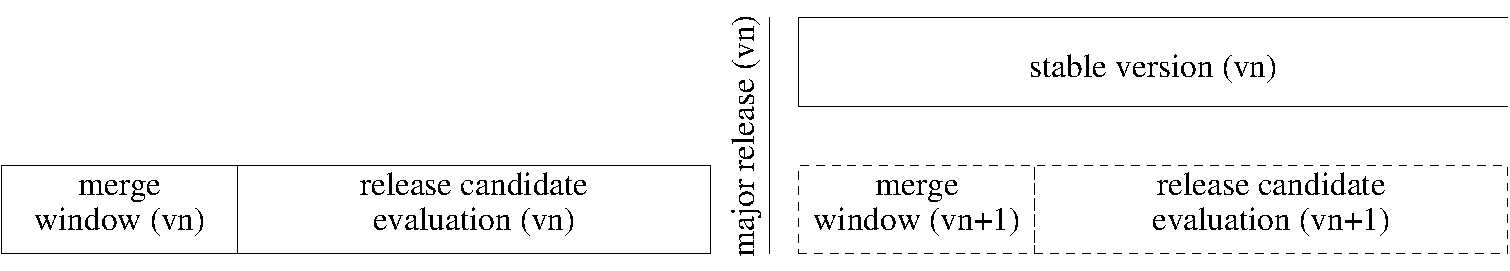
\includegraphics[width=\linewidth]{versions.pdf}\]
\caption{Four phases of Linux development}
\label{devmodel}
\end{figure}

The Linux kernel development model introduces some delay between when new
features are developed and when they are integrated into a release
candidate or major release.  To compensate for this delay, the
linux-next\footnote{git://git.kernel.org/pub/scm/linux/kernel/git/next/linux-next.git}
tree is used to mimic the merge window on daily basis, by pulling from each
subsystem tree. Every day the tree is reset to the latest major
kernel release and then each subsystem tree is pulled. The linux-next tree
can thus be used to track the latest development efforts on all subsystems on a
daily basis.

\subsection{A brief history of the Linux kernel backports project}

The Linux kernel backports
project\footnote{https://backports.wiki.kernel.org} was started in 2007 by
Luis R. Rodriguez while at Rutgers University, originally to help backport
the 802.11 subsystem and a series of 802.11 device drivers to a series of
older kernel
releases.\footnote{git://git.kernel.org/pub/scm/linux/kernel/git/mcgrof/compat-wireless-2.6-old.git}
The project was originally referred to as {\em compat-wireless}, reflecting
the initial target.  Over the years, the project grew to support more
device drivers and subsystems. In April 2012, at the Linux Collaboration
summit in San Francisco it was decided to rebrand the project {\em
  compat-drivers}\footnote{git://git.kernel.org/pub/scm/linux/kernel/git/mcgrof/compat-drivers-old.git}
when the project was folded under the Linux Foundation backports working
group.\footnote{http://lists.linuxfoundation.org/pipermail/lf\_driver\_backport/2012-August/001075.html}
The project now spearheads the Linux kernel backports effort. The last
rebranding of the project happened in April 2013, when it took on the name
{\em backports}, to distinguish it from the Linux kernel compat layer,
which addresses 64-bit and 32-bit compatibility.  The backports project is
now led by three core developers: Hauke Mehrtens, Johannes Berg,
Luis Rodriguez; two co-maintainers: Hauke and Luis; and is developed
and supported by a series of contributors.  It backports the subsystems Ethernet,
Wireless, Bluetooth, NFC, ieee802154, Media, and Regulator.

%% v2.6.30 - v3.6 - compat-wireless
%% v3.7 - v3.9 - compat-drivers
%% v3.10 - on - backports

The current goal of the backports project is to backport a slew of device
drivers from the latest major kernel releases down to a series of supported
stable kernel releases, at a minimum those listed on the main kernel
website, {\tt kernel.org}.  Currently, 18 releases are supported.  The
project's master development branch always tracks linux-next, allowing it
to track all the development trees. This ensures that at the end of each
merge window, the state of the backports will be very close to the state of
the first release candidate.  At this point, the backports project creates
a further branch that tracks the progress of the new release over the
release candidate evaluation period, to the major release, and on to its
lifetime as a stable kernel.  The backports project thus makes three kinds
of backports available: those derived from linux-next, those derived from
the most recent release candidate if any, and those derived from recent
stable kernels.  A user may prefer a backport from a stable kernel to one
from linux-next or from a release candidate, if one is available for the
desired driver.

As shown in Figure \ref{num}, as of September 2014, the backports project
backports almost 800 drivers.  These are kept up to date with linux-next
and the recent stable kernels each day, and are guaranteed to at least
compile correctly. Ensuring this each day typically requires 2-6 iterations
of test, refinements, and compiles for all supported versions. For this
development, the backports project uses a 32-core system with 236 GiB of
RAM.  Code generation and compile tests are all run in memory. As measured
by GNU {\tt time}, a full compilation test of a release across all 18
supported kernel revisions takes approximately 22 minutes of real time, 744
minutes of user mode time and 83 minutes of kernel time.  When the
backports project began in 2007, it provided backporting support for
drivers down to v2.6.25, first released in 2008. In order to scale to a
wider range of drivers, however, the project now only supports kernels down
to at most Linux v3.0, first released in 2011. The original motivation
behind the project was to encourage silicon manufacturers to work upstream
on the Linux kernel while providing them a solution for backporting their
drivers automatically down to older releases.  The framework is designed
{\em only} for Linux upstream drivers; the associated license enforces that
proprietary drivers cannot and should not use this framework.

\begin{figure}
\[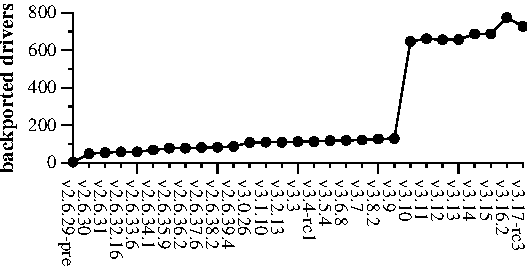
\includegraphics{supported.pdf}\]
\caption{Number of backported drivers, for kernels released since
  2009}
\label{num}
\end{figure}

\subsection{Coccinelle}

Coccinelle is a program matching and transformation engine for C code
\cite{Padioleau:eurosys08,Brunel:POPL09}.  It is released as open source,
and is available in a number of Linux distributions.  Coccinelle provides a
scripting language, SmPL ({\em semantic patch language}), that allows
patterns to be expressed as fragments of C code, and transformations to be
expressed by annotating lines of code with \verb+-+, for removal of the
matched code, or \verb-+-, for addition of the corresponding code.  As
such, SmPL specifications resemble {\em patches} \cite{diffmanual:02}.
Nevertheless, they are more robust than ordinary patches in that they are
insensitive to comments and whitespace, and take into account some aspects
of the code semantics such as control flow and type information.
Thus, we refer to SmPL specifications as {\em semantic patches}.

As a simple example of the use of Coccinelle, we consider the problem of
replacing all calls to a function named {\tt one} by calls to a function
named {\tt two}, and adding a {\tt NULL} argument.  The semantic patch that
makes this change is shown in Figure \ref{fig:sp1}.  This semantic patch
consists of a single rule that makes the complete transformation.  The rule
is in two parts: the declaration of {\em metavariables} that can match any
term of a specified type between the initial pair of {\tt @@} (lines 1-3),
followed by a {\em transformation specification} (lines 4-5).  In this
case, the only metavariable is {\tt arg}, which is declared to match any
expression.  The transformation specification then removes the call to {\tt
  one} with its argument, while at the same time binding the metavariable
{\tt arg} to this argument expression.  It then constructs a new function
call to the function {\tt two} with arguments the current binding of {\tt
  arg} and {\tt NULL}.  This semantic patch can be applied to an entire
code base.  A more detailed presentation of Coccinelle is available in
previous work \cite{Padioleau:eurosys08,Brunel:POPL09} and at the
Coccinelle website.\footnote{http://coccinelle.lip6.fr}

\begin{figure}
\begin{lstlisting}[language=diff]
@@
expression arg;
@@
- one(arg)
+ two(arg, NULL)
\end{lstlisting}
\caption{A simple semantic patch}
\label{fig:sp1}
\end{figure}

Coccinelle was originally motivated by a study of how the Linux kernel
evolves \cite{Padioleau:eurosys06}.  This study identified the problem of
{\em collateral evolutions}, in which the interface of a library changes,
and all clients of the library must be updated accordingly.  Coccinelle was
designed to help Linux developers make collateral evolutions faster and
more reliably.  The problem of implementing backports using Coccinelle is
related to the problem of collateral evolutions.  While collateral
evolutions were envisioned as being needed to modernize software, backports
must address changes in library interfaces to transport modern code to
older versions.

%% Furthermore, in practice even an aggressive
%% developer may only need to perform a collateral evolution infrequently,
%% perhaps once or twice a month. The use case for backports is very
%% different.  The code that has to be backported changes daily, via updates
%% in linux-next.  Thus, Coccinelle would have to be used daily, with all
%% semantic patches being applied against all supported subsystems and
%% drivers.


\section{Backporting strategies}
\label{strategies}

We now review three backporting strategies: i) the common strategy of
providing version-specific implementations using \#ifdefs, ii) the strategy
originally taken by the Linux backports project of factorizing these
changes into a compatibility library, and iii) our extension of the latter
using Coccinelle.

\subsection{Backporting with \#ifdefs}

Backporting a device driver typically consists of modifying the source code
with \#ifdefs to handle the different requirements of different kernel
releases.  This entails adding blocks of code that provide alternate
implementations for various functionalities, for different ranges of kernel
versions, according to which evolutions have occurred and which collateral
evolutions must be performed to accommodate them.

As a running example, we consider an evolution that was introduced by Linux
kernel commit d314774cf2 and that was first merged upstream in Linux
v2.6.29.  This evolution moved a series of callback functions from the {\tt
  net\_\-device} data structure out into a new separate data structure of
type {\tt net\_\-device\_\-ops}.  Backporting over this evolution, for Linux
kernel versions before Linux v2.6.29, requires collateral evolutions that
{\em undo} this change.  Specifically, the definition of the new {\tt
  net\_\-device\_\-ops} structure and the initialization of the link from the
{\tt net\_\-device} structure to this new structure must be restricted, using
an \#ifdef, to the versions starting with Linux v2.6.29.  Earlier versions
must initialize the appropriate fields in the {\tt net\_\-device} structure
itself, from among the callback functions that the modern driver puts in the
new structure.  Figure \ref{usbport} shows a patch that backports this
single collateral evolution on one device driver.

\begin{figure}
\begin{lstlisting}[language=diff]
--- a/drivers/net/usb/usbnet.c
+++ b/drivers/net/usb/usbnet.c
@@ -1151,6 +1151,7 @@
 }
 EXPORT_SYMBOL_GPL(usbnet_disconnect);
 
+#if (LINUX_VERSION_CODE >= KERNEL_VERSION(2,6,29))
 static const struct net_device_ops usbnet_netdev_ops = {
   .ndo_open               = usbnet_open,
   .ndo_stop               = usbnet_stop,
@@ -1160,6 +1161,7 @@
   .ndo_set_mac_address    = eth_mac_addr,
   .ndo_validate_addr      = eth_validate_addr,
 };
+#endif
 
 /*-----------------------------------------------------*/
 
@@ -1229,7 +1231,15 @@
     net->features |= NETIF_F_HIGHDMA;
 #endif
 
+#if (LINUX_VERSION_CODE >= KERNEL_VERSION(2,6,29))
   net->netdev_ops = &usbnet_netdev_ops;
+#else
+  net->change_mtu = usbnet_change_mtu;
+  net->hard_start_xmit = usbnet_start_xmit;
+  net->open = usbnet_open;
+  net->stop = usbnet_stop;
+  net->tx_timeout = usbnet_tx_timeout;
+#endif
   net->watchdog_timeo = TX_TIMEOUT_JIFFIES;
   net->ethtool_ops = &usbnet_ethtool_ops;
\end{lstlisting}
\caption{Backporting the {\tt net\_\-device\_\-ops} collateral evolution for
  the {\tt usbnet} driver}
\label{usbport}
\end{figure}

Lines 7 and 23 of Figure \ref{usbport} introduce the \#ifdefs that restrict
some code of the modern driver to be used only in Linux versions v2.6.29
and later.  Lines 25-31 introduce the code to be used for earlier versions,
placing the relevant callback functions from the modern code (lines 8-13)
into the fields of the {\tt net} structure.  In each case, the callback
functions are used by the driver support library of the kernel, which is
not backported, and which thus finds the desired functions in the expected
place, with no further code changes.

In general, every driver that initializes a {\tt net\_\-device} structure
would require all of these changes.  Creating these patches, and
maintaining them as other collateral evolutions are needed, is complex,
tedious, and error prone.
%\jl{Who uses this approach?}

\subsection{Backports via a compatibility library}

Maintenance of patches is easy as long as the amount of changes being
introduced is rather small. The {\tt netdev\_\-ops} collateral evolution,
however, is an example of a collateral evolution that affects many network
drivers, resulting in a large set of changes, that then have to be
maintained in patch form.  A better approach, proposed by the Linux
backports project, consists of wrapping up the required changes into static
inline or external helper functions and then using \#ifdefs in these
functions to adapt the code to each previous release.

This strategy is illustrated by the following code, which backports the
{\tt netdev\_\-ops} collateral evolution for two device drivers.  Now, the
new {\tt net\_\-device\_\-ops} structure used by the modern driver is
maintained as is.  Instead, we replace the direct initialization of the
{\tt netdev\_\-ops} field by a call to a single static inline function
defined by the backports compat library, amounting to glue code.  Now, only
this function needs multiple lines of \verb-#ifdef- code, performing the
direct assignment for versions starting with Linux v2.6.29, and copying the
fields from the new structure into the main {\tt net\_\-device} structure
for the older versions.  Only one line of code is changed in each driver,
in contrast to the 10 lines added to each driver by the previous approach.

\begin{lstlisting}[language=diff]
--- a/drivers/net/usb/usbnet.c
+++ b/drivers/net/usb/usbnet.c
@@ -1446,7 +1446,7 @@ usbnet_probe (struct usb_interface *udev
     net->features |= NETIF_F_HIGHDMA;
 #endif
 
-  net->netdev_ops = &usbnet_netdev_ops;
+  netdev_attach_ops(net, &usbnet_netdev_ops);
   net->watchdog_timeo = TX_TIMEOUT_JIFFIES;
   net->ethtool_ops = &usbnet_ethtool_ops;
 
--- a/drivers/net/wireless/ath/ath6kl/main.c
+++ b/drivers/net/wireless/ath/ath6kl/main.c
@@ -1289,7 +1289,7 @@ static const struct net_device_ops ath6k
 
 void init_netdev(struct net_device *dev)
 {
-  dev->netdev_ops = &ath6kl_netdev_ops;
+  netdev_attach_ops(dev, &ath6kl_netdev_ops);
   dev->destructor = free_netdev;
   dev->watchdog_timeo = ATH6KL_TX_TIMEOUT;
\end{lstlisting}

Between 2007 and 2013 the backports project exclusively followed this
strategy to help reduce the amount of maintenance on patches. The backport
compat library now has a large set of helper functions that help to keep the
number and size of the patches required for each backported driver to a
minimum.

\subsection{The Coccinelle way to backport}

The compat library approach reduces significantly the amount of code that
must be modified in each driver. Still, backporting a new driver requires
identifying the set of features that it uses, and comparing these features
to those provided by the compat library to see where a collateral evolution
to replace the existing code by glue code invoking the compat library is
needed.  Just as Coccinelle had been found to be useful in performing
traditional (forward) collateral evolutions, we considered whether
Coccinelle could also be useful for the kinds of collateral evolutions
required in backports. For example, the {\tt netdev\_\-ops} collateral
evolution could be expressed as a Coccinelle semantic patch as follows:

\begin{lstlisting}[language=diff]
@@
struct net_device *dev;
struct net_device_ops ops;
@@
- dev->netdev_ops = &ops;
+ netdev_attach_ops(dev, &ops);
\end{lstlisting}

This semantic patch could be used to backport the netdev\_\-ops collateral
evolution for all networking device drivers.  It is indeed no longer even
necessary for the developer to identify whether a new device driver to
backport uses this features; Coccinelle both finds and updates the relevant
code automatically.  Note in particular that the semantic patch specifies
the type of the expressions matching the {\tt dev} and {\tt ops}
metavariables, to ensure that the transformation is performed only on
structures of the appropriate type.  Finally, this semantic patch amounts to
only 6 lines of code to maintain, rather than 2 lines of code {\em for each
  driver} with the \#ifdef approach.

\section{Case Study}
\label{case}

To test the limits of what can be backported using Coccinelle, we chose the
most complex collateral evolution supported by the backports project as a
test case.  Specifically, we decided to try to backport threaded IRQ
support, introduced in the v2.6.31 kernel.  This backport requires
modifications to a driver-specific structure, as well as to multiple driver
functions.

\subsection{Backporting threaded IRQ support the old way}

We first explain how the backports project provided backport support for
threaded IRQ support prior to the use of Coccinelle.  The first step was to
extend the compat library with support for threaded IRQs, as shown in
Figure \ref{compat}.  This involved creating a new data type {\tt
  compat\_\-threa\-ded\_\-irq} (lines 1-11) to collect some extra information
for each driver, and creating a set of helper functions to implement the
threaded IRQ fuctionality (lines 13-69).  The helper functions include {\tt
  compat\_\-request\_\-threa\-ded\_\-irq} (lines 26-44), which initializes
the fields of the {\tt compat\_\-threa\-ded\_\-irq} structure and then calls
{\tt request\_\-irq}, and functions such as {\tt
  compat\_\-free\_\-threa\-ded\_\-irq} (lines 46-51) and {\tt
  compat\_\-synchronize\_\-threa\-ded\_\-irq} (lines 62-69) that call their
unthreaded counterparts on information stored in the {\tt
  compat\_\-threa\-ded\_\-irq} structure.  In all, the extension to the
compat library amounts to 75 lines of code.\footnote{Computed using David
  Wheeler's SLOCCount, \newline http://www.dwheeler.com/sloccount/.}

%% 10 for structure, 65 for functions
%% The complete code is in compat_extend.c

\begin{figure}[h!]
\begin{lstlisting}[language=C]
#if LINUX_VERSION_CODE < KERNEL_VERSION(2,6,31)
struct compat_threaded_irq {
	unsigned int irq;
	irq_handler_t handler;
	irq_handler_t thread_fn;
	void *dev_id;
	char wq_name[64];
	struct workqueue_struct *wq;
	struct work_struct work;
};
#endif

#if LINUX_VERSION_CODE < KERNEL_VERSION(2,6,31)
static inline
void compat_irq_work(struct work_struct *work)
{
  ...
}

static inline
irqreturn_t compat_irq_dispatcher(int irq, void *dev_id)
{
  ...
}

static inline
int compat_request_threaded_irq(
	struct compat_threaded_irq *comp,
	unsigned int irq,
	irq_handler_t handler,
	irq_handler_t thread_fn,
	unsigned long flags,
	const char *name,
	void *dev_id)
{
  comp->irq = irq;
  comp->handler = handler;
  comp->thread_fn = thread_fn;
  comp->dev_id = dev_id;
  INIT_WORK(&comp->work, compat_irq_work);
  ...
  return request_irq(irq, compat_irq_dispatcher, flags,
		 name, comp);
}

static inline
void compat_free_threaded_irq(
	struct compat_threaded_irq *comp)
{
  free_irq(comp->irq, comp);
}

static inline
void compat_destroy_threaded_irq(
	struct compat_threaded_irq *comp)
{
  if (comp->wq)
    destroy_workqueue(comp->wq);
  comp->wq = NULL;
}

static inline
void compat_synchronize_threaded_irq(
	struct compat_threaded_irq *comp)
{
  synchronize_irq(comp->irq);
  cancel_work_sync(&comp->work);
}
#endif
\end{lstlisting}
\caption{Extensions to the compat library to support \newline {\tt
    request\_\-threa\-ded\_\-irq}}
\label{compat}
\end{figure}

Each driver to backport that relies on threaded IRQs then needs to be
modified to make use of the new helper functions.  Figure \ref{compatpatch}
shows the modifications for the b43 driver.  Lines 1-13 update a header
file to extend the driver's private {\tt b43\_\-wldev} structure type with
a field containing the compat structure when the kernel version is lower
than the first one that supports threaded irqs.  Lines 14-52 replace each
threaded IRQ operation with its compat version, again for kernels for which
threaded irqs are not already supported.

\begin{figure}
\begin{lstlisting}[language=diff]
--- a/drivers/net/wireless/b43/b43.h
+++ b/drivers/net/wireless/b43/b43.h
@@ -805,6 +805,9 @@ enum {
 
 /* Data structure for one wireless device (802.11 core) */
 struct b43_wldev {
+#if LINUX_VERSION_CODE < KERNEL_VERSION(2,6,31)
+	struct compat_threaded_irq irq_compat;
+#endif
 	struct b43_bus_dev *dev;
 	struct b43_wl *wl;
 	/* a completion event structure needed if this call is
            asynchronous */
--- a/drivers/net/wireless/b43/main.c
+++ b/drivers/net/wireless/b43/main.c
@@ -4243,8 +4243,17 @@ redo:
 	if (b43_bus_host_is_sdio(dev->dev)) {
 		b43_sdio_free_irq(dev);
 	} else {
+#if LINUX_VERSION_CODE >= KERNEL_VERSION(2,6,31)
 		synchronize_irq(dev->dev->irq);
+#else
+		compat_synchronize_threaded_irq(&dev->irq_compat);
+#endif
+#if LINUX_VERSION_CODE >= KERNEL_VERSION(2,6,31)
 		free_irq(dev->dev->irq, dev);
+#else
+		compat_free_threaded_irq(&dev->irq_compat);
+		compat_destroy_threaded_irq(&dev->irq_compat);
+#endif
 	}
 	mutex_lock(&wl->mutex);
 	dev = wl->current_dev;
@@ -4290,9 +4299,17 @@ static int b43_wireless_core_start(
 			goto out;
 		}
 	} else {
+#if LINUX_VERSION_CODE >= KERNEL_VERSION(2,6,31)
                err = request_threaded_irq(dev->dev->irq,
				b43_interrupt_handler,
				b43_interrupt_thread_handler,
				IRQF_SHARED, KBUILD_MODNAME, dev);
+#else
+               err = compat_request_threaded_irq(&dev->irq_compat,
+					dev->dev->irq,
+					b43_interrupt_handler,
+					b43_interrupt_thread_handler,
+					IRQF_SHARED, KBUILD_MODNAME, dev);
+#endif
 		if (err) {
 			b43err(dev->wl, "Cannot request IRQ-%d\n",
 			       dev->dev->irq);
\end{lstlisting}
\caption{Backporting the b43 driver}
\label{compatpatch}
\end{figure}

The changes shown in Figure \ref{compatpatch} amount to 20 lines of added
code and only apply to a single driver.  As of the linux-next of October
15, 2014, 169 files contain at least one call to {\tt
  request\_\-threa\-ded\_\-irq}, and of these 16 are in subsystems supported
by the Linux backports project.\footnote{1 in ethernet, 7 in wireless, 0 in
  bluetooth, 2 in nfc, 0 in ieee802145, 4 in media, 2 in regulator.}
Backporting all of the 169 files that use threaded IRQs to Linux versions
prior to v2.6.31 would require developing and maintaining over 3000 lines
of patch code.

\subsection{Backporting threaded IRQ support with Coccinelle}

Figure \ref{thrdirq} shows a Coccinelle semantic patch that automates these
changes.  Most are relatively trivial: replace one call with another,
with the new call using the backport data structure among its arguments.  A
typical example is illustrated in the first rule (lines 1-24), where a call
to {\tt request\_\-threa\-ded\_\-irq} is replaced by a call to {\tt
  compat\_\-request\_\-threa\-ded\_\-irq}.  The new call takes the same
arguments as the old one, with the addition of the
first argument (line 17), which is the {\tt compat\_\-threa\-ded\_\-irq}
structure.

\begin{figure}
\begin{lstlisting}[language=diff]
@ threaded_irq @
identifier ret;
expression irq, irq_handler, irq_thread_handler, flags,
           name;
type T;
T *private;
@@

+#if LINUX_VERSION_CODE >= KERNEL_VERSION(2,6,31)
ret = request_threaded_irq(irq,
			   irq_handler,
			   irq_thread_handler,
			   flags,
			   name,
			   private);
+#else
+ret = compat_request_threaded_irq(&private->irq_compat,
+				   irq,
+				   irq_handler,
+				   irq_thread_handler,
+				   flags,
+				   name,
+				   private);
+#endif

@ sync_irq depends on threaded_irq @
expression irq;
type threaded_irq.T;
T *threaded_irq.private;
@@

+#if LINUX_VERSION_CODE >= KERNEL_VERSION(2,6,31)
synchronize_irq(irq);
+#else
+compat_synchronize_threaded_irq(&private->irq_compat);
+#endif

@ free depends on threaded_irq @
expression irq, dev;
type threaded_irq.T;
T *threaded_irq.private;
@@

+#if LINUX_VERSION_CODE >= KERNEL_VERSION(2,6,31)
free_irq(irq, dev);
+#else
+compat_free_threaded_irq(&private->irq_compat);
+compat_destroy_threaded_irq(&dev->irq_compat);
+#endif

@ modify_private_header depends on threaded_irq @
type threaded_irq.T;
@@

T {
+#if LINUX_VERSION_CODE < KERNEL_VERSION(2,6,31)
+      struct compat_threaded_irq irq_compat;
+#endif
...
};
\end{lstlisting}
\caption{Backporting threaded IRQs with Coccinelle}
\label{thrdirq}
\end{figure}

A challenge in implementing this backport is where to store the {\tt
  compat\_\-threa\-ded\_\-irq} structure.  As multiple instances of a device
may be present in a running kernel, this structure cannot simply be a
global variable of the device driver.  In the case of the b43 driver, we
placed this structure into the driver's {\tt b43\_\-wldev} structure.  To
generalize this, we need to find a suitable location for this structure in
each driver to which the semantic patch may be applied.

The need to support multiple instances of a data structure at run time is a
common problem in device driver development, and the Linux kernel proposes
a standard solution, the use of a {\em private} data structure.  An
instance of this private structure is created when a device is initialized,
and then the driver infrastructure makes this structure available to each
driver callback function, much like the implicit ``this'' argument found in
object-oriented languages.  Normally, each driver defines a specific
private-structure type, containing the information that is specific to its
operation.  We exploit this private structure to store the {\tt
  compat\_\-threa\-ded\_\-irq} structure.

To use the private structure to store the {\tt compat\_\-threa\-ded\_\-irq}
structure, we must address two issues.  First, for each driver, we must
find the type of the private structure and extend the corresponding type
declaration with a field for the {\tt compat\_\-threa\-ded\_\-irq} structure.
Second, we must find the name of the current instance of the private
structure at each point where a reference to the {\tt
  compat\_\-threa\-ded\_\-irq} structure is needed for the backport process.

To address the first issue, we exploit the fact that Coccinelle collects
type information when analyzing the source code, and makes it possible to
manipulate this type information via metavariables in a semantic patch.
Fortunately, device drivers typically already pass their private structure
as the last argument to {\tt request\_\-threa\-ded\_\-irq}, as the
information contained in the private structure is typically also needed by
the interrupt handler, which is installed by this function.  By matching
this reference to the private structure, Coccinelle makes it possible to
obtain its type.  Concretely, line 5 of Figure \ref{thrdirq} declares a
type metavariable {\tt T}, which is then used in describing the type of
metavariable {\tt private}.  Matching {\tt private} against the code in the
last argument of {\tt request\_\-threa\-ded\_\-irq} has the side effect of
storing the type of the matched code in {\tt T}, where it can be used by
subsequent rules.  In the fourth rule (lines 51 to 60), {\tt T}, referenced
as {\tt threaded\_\-irq.T}, is used to match and extend the definition of
the private structure, adding a new field {\tt irq\_\-compat} to the
beginning of the private structure when the kernel version is less than
v2.6.31.

To address the second issue, we exploit the fact that, within a given
driver, the Linux developers typically give the private structure the same
name, in every function in which it is used.  Thus, we simply inherit the
term matched by the metavariable {\tt private} defined in the rule {\tt
  threaded\_\-irq}, and use that term in the added calls in the {\tt
  synch\_\-irq} and {\tt free} rules.  This solution is not safe, but it is
pragmatic, in that it simplifies the transformation and exploits properties
of the Linux coding style.  Note that in the {\tt free\_\-irq} case (lines
38-49), we could also use the second argument to {\tt free\_\-irq}, which
by definition of the IRQ API should point to the same structure as the last
argument to {\tt request\_\-threa\-ded\_\-irq}.\footnote{Actually,
  unintentionally, in the second call that is added by this rule, this
  strategy is used.}  This value is not immediately available in the {\tt
  sync\_\-irq} rule (lines 26-36), but we could extend the rule to match a
neighboring expression of the right type, for a safer solution.

\subsection{Benefits of using Coccinelle for backporting}

Reimplementing the threaded IRQ backport using Coccinelle revealed that the
original manual backport was inconsistent.  Specifically, in the manual
backport, the compat structure, {\tt compat\_\-thread\_\-irq}, was integrated
into different structures in different drivers.  Backporting is
intrinsically risky, because the older code may not respect the invariants
required by the backported code.  Modifying the older code in a consistent
way reduces the set of issues that can arise.  Doing so also
makes the results easier for developers to understand.

Reimplementing the threaded IRQ backport using Coccinelle also revealed
that the existing threaded IRQ patch series also backported another
collateral evolution, related to the management of IRQ flags.  Isolating
each collateral evolution in a separate patch benefits the backports
project, by making it easier to understand how to backport other drivers,
which may need only one of the changes.  Using Coccinelle not only makes
the need for this split apparent, it also makes it easier to manage the
resulting set of changes.  While two sets of changes are now needed, each
is performed by a single semantic patch that can be applied to many files,
rather than having to implement and record each of the changes
individually.

Finally, for a few patch series, the amount of time to generate a
backported release was actually reduced, as compared to the application of
the manually created patches.  Coccinelle has to parse the driver C code
and search for relevant code, all of which are much more expensive than
applying a patch, in which the file name, line number, and code context are
explicitly specified.  Nevertheless, patch application is sequential, while
Coccinelle can work on a collection of individual files in parallel.  This
difference is sufficient to make the use of Coccinelle faster in some
cases.


\section{Correctness and Performance}
\label{correct}

We now consider some correctness and performance issues raised by the use
of Coccinelle.

\subsection{Correctness}

For the traditional uses of Coccinelle, for bug finding and collateral
evolutions, a developer runs Coccinelle once on a code base, checks and
possibly adjusts the results, and submits a patch upstream for review by
kernel maintainers.  The patch is integrated into the Linux kernel just
like a manually generated patch, and Coccinelle is no longer involved.

The use case for backports is rather different.  Here, the developer
typically starts with a collection of patches, reflecting the result of
backporting a number of drivers by hand.  The developer then generalizes
the existing patches into a semantic patch, which is then applied every
day, as linux-next and the various stable kernels evolve.  In this context,
manually studying each result is not practical, and would likely not be
reliable.  Still, it is necessary to account for the possibility of errors,
either in the semantic patch definition or in Coccinelle itself.  Indeed,
some improvements to Coccinelle were required to enable its use for
backporting, such as improving the support for adding \#ifdefs around
complete function definitions.

To check the correctness of the result of Coccinelle, we exploit the
existence of manually developed patches that perform the desired
transformation.  Specifically, we have developed a simple tool that applies
the manually developed patches and the semantic patches to separate copies
of the Linux kernel source code, and then checks that the results are
equal.
%
After applying the semantic patches to a possible target release and
comparing the result with that of applying the manually written backport
patches, we were surprised to find that the semantic patches produced more
code changes.  Indeed, the functionalities backported by the semantic
patches occur in drivers that, while they are integrated on Linux
backports, are not yet enabled for older kernels, as they require
backporting of more collateral evolutions. A semantic patch transforms all
code that exhibits the specified pattern, and thus generalizing a backport
with Coccinelle can extend that backport to more drivers. Once all of the
collateral evolutions required by a particular driver for a given kernel
have been implemented, then that driver can be enabled for use on that
kernel.  When all required collateral evolutions to support a given kernel
have been addressed with Coccinelle, then new drivers can be backported to
that kernel fully automatically.

%% Since git is prevalent on the target directories where we typically
%% want to do changes I just use git, and what I do is apply the legacy
%% patch first, commit that. Then I apply the inverse of the patch but do
%% not commit that, and then I apply the SmPL patch. All + stuff is
%% things that is extra, all - stuff is stuff that is removed. This is
%% how I found out about the different collateral evolution that we
%% tugged along into the original patch series.


\subsection{Performance}

Each day, the Linux kernel backports project generates and compile tests
backport releases for all supported kernels, of which there are currently
18.  Generation for all of them takes around 2 minutes on our 32-core
machine, and compile testing of the 18 resulting patched kernels takes 40
minutes of real time, comprising 1086 minutes of user time and 139 minutes
of system time.  Given the long compilation time, it is important to
minimize the time for generating backports.  Several solutions were
explored to avoid the use of Coccinelle overwhelming the backporting time.
Figures \ref{num_patches} and \ref{small_num} relate the backport
generation time to the number of supported kernels, patches, and resulting
backported drivers for recent kernels.

%% real    40m15.411s
%% user    1085m54.776s
%% sys     139m23.312s

%% This is across these 18 kernels (including v3.17, but obviously we
%% should skip that):

%% 1   3.0.101             [  OK  ]
%% 2   3.1.10              [  OK  ]
%% 3   3.2.62              [  OK  ]
%% 4   3.3.8               [  OK  ]
%% 5   3.4.103             [  OK  ]
%% 6   3.5.7               [  OK  ]
%% 7   3.6.11              [  OK  ]
%% 8   3.7.10              [  OK  ]
%% 9   3.8.13              [  OK  ]
%% 10  3.9.11              [  OK  ]
%% 11  3.10.54             [  OK  ]
%% 12  3.11.10             [  OK  ]
%% 13  3.12.27             [  OK  ]
%% 14  3.13.11             [  OK  ]
%% 15  3.14.18             [  OK  ]
%% 16  3.15.10             [  OK  ]
%% 17  3.16.2              [  OK  ]
%% 18  3.17-rc3            [  OK  ]


%% For this, the project uses a
%% 32-core server donated by HP, SUSE and the Linux Foundation, having 236 GiB
%% RAM.  The project uses a /pub/mem tmpfs, allowing it to have the upstream
%% Linux kernel git tree and the stable kernel git tree,\footnote{The
%%   linux.git and linux-stable.git git trees from kernel.org, respectively.}
%% the backport patches and the compat library, and all of the generated code
%% in RAM. Compilation tests are all performed in RAM.  Prior to the use of
%% Coccinelle, the compilation time dominated the daily tasks involved in
%% backporting.  Applying a semantic patch involves parsing and processing
%% source code, and is thus much more expensive than simple line-by-line patch
%% application.  Several solutions were explored to avoid the use of
%% Coccinelle overwhelming the backporting time.

\begin{figure}
\[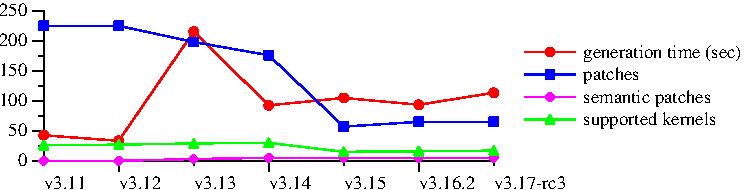
\includegraphics[width=\linewidth]{patchtimes.pdf}\]
\caption{Generation time compared to number of patches, semantic patches,
  and supported kernel versions}
\label{num_patches}
\[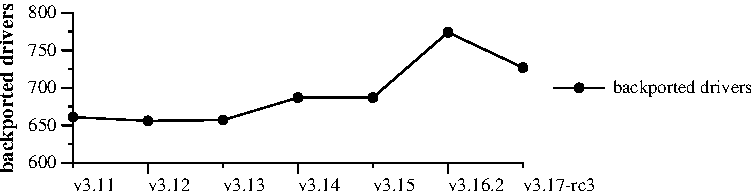
\includegraphics[width=\linewidth]{small_supported.pdf}\]
\caption{Number of backported drivers, for recent kernels}
\label{small_num}
\end{figure}

As a first try, in v3.13, all of the semantic patches were concatenated and
run in a single thread, much like the application of standard patches.  In
a uniprocessor environment, this avoids the cost of starting up Coccinelle
for each semantic patch.  This solution, however, does not exploit the
parallelism inherent in applying a single specification to the hundreds of
drivers supported by the backports project, and we see a high generation
time in Figure \ref{num_patches} for v3.13.  Coccinelle currently supports
static parallelism via an external script that starts up $n$ instances of
Coccinelle and causes each of them to process $1/n$ of the files in the
code base.  Performance can further be improved by instructing Coccinelle
to use index information, precollected by a tool such as
glimpse,\footnote{http://webglimpse.net/.  As a side effect of this work,
  the first author convinced the developers of glimpse to release glimpse
  as open source.} to identify the subset of files that may be relevant to
a given semantic patch.  With these two optimizations, semantic patch
support can be less expensive than sequential application of the
corresponding patches.  For example, for v3.26.2, the number of supported
drivers increases significantly (Figure \ref{small_num}), but the generation
time actually slightly goes down.  Currently, we are exploring the
integration of parallelism into Coccinelle itself using the OCaml library
Parmap \cite{Danelutto:12}, which provides dynamic scheduling.  Preliminary
tests suggest that this will improve CPU utilization and yield further
performance improvements.

%% \subsection{Coccinelle Parallelizing improvements}

%% The backports project ended up fine tuning usage of Coccinelle
%% with sensible arguments and managing Coccinelle's current parallelism
%% support using Python. The script was generalized for regular
%% kernel development and is now merged on Coccinelle development
%% git tree. It is used as follows:

%% \begin{lstlisting}[language=bash]
%% pycocci foo.cocci drivers/
%% \end{lstlisting}

%% This script causes Coccinelle to make changes in place in the source code
%% (Coccinelle option {\tt -{}-in-place}, it is parallelized, and a number of
%% other sensible command-line arguments are provided if one wants to apply
%% rules broadly. In the future, Coccinelle will be modified to use the OCaml
%% Parmap library for integrated parallelism support. In order to help make
%% Coccinelle run faster software index utilities can be used, glimpse is one
%% option, another is idutils. Glimpse is unfortunately not FOSS. By default
%% Coccinelle relies on its own grep implementation to search for tokens.

\subsection{Further improvements: a needle in a haystack}

Coccinelle applies the rules of a semantic patch in order, from first to
last, with any changes specified by a rule being performed as soon as
the rule is matched.  This can lead to extra matching and undesired
modifications if rules that perform generic transformations are placed at
the beginning of a semantic patch.  As an example, consider the following
rule that begins a semantic patch for backporting PCI drivers:

\begin{lstlisting}[language=diff]
@ simple_dev_pm depends on module_pci @
identifier ops, pci_suspend, pci_resume;
declarer name SIMPLE_DEV_PM_OPS;
declarer name compat_pci_suspend;
declarer name compat_pci_resume;
@@
+compat_pci_suspend(pci_suspend);
+compat_pci_resume(pci_resume);
SIMPLE_DEV_PM_OPS(ops, pci_suspend, pci_resume);
\end{lstlisting}

%% In the following 419 comes from searching for SIMPLE_DEV_PM_OPS, and 61
%% comes from additionally looking for the declaration and initialization
%% of a pci_driver structure.  See misc/pcipm.cocci on palace.

\noindent
This rule collects some information from each {\tt
  SIMPLE\_\-DEV\_\-PM\_\-OPS} structure, and introduces some PCI-specific
calls from the compat library.  The rule applies to every {\tt
  SIMPLE\_\-DEV\_\-PM\_\-OPS} declaration, and is not specific to PCI
drivers in any way.  Not only does it transform code that should not be
transformed, it also can potentially have a significant performance impact.
In the linux-next of October 15, 2014, there are 419 files that contain a
{\tt SIMPLE\_\-DEV\_\-PM\_\-OPS} declaration, while only 61 of these are
PCI drivers.  All of these extra files will be parsed and (unnecessarily)
transformed if the semantic patch is written in this way.

A solution is to add a rule that matches against some other more specific
term that must be present if any transformation is to be performed.  Other
rules can then depend on the success of matching this rule.  Essentially,
this rule acts as a ``needle in a haystack'' to find the source files
where the transformation is actually relevant.  In this particular case, we
observe that PCI drivers contain a {\tt MODULE\_\-DEVICE\_\-TABLE}
declaration with {\tt pci} as the first argument. We thus add the following
rule at the beginning of the semantic patch:

\begin{lstlisting}[language=diff]
@ module_pci @
declarer name MODULE_DEVICE_TABLE;
identifier pci_ids;
@@
MODULE_DEVICE_TABLE(pci, pci_ids);
\end{lstlisting}

The {\tt SIMPLE\_\-DEV\_\-PM\_\-OPS} rule can now be declared to depend on
the rule {\tt module\_\-pci}, ensuring that it is only applied to PCI
drivers:

\begin{lstlisting}[language=diff]
@ simple_dev_pm depends on module_pci @
identifier ops, pci_suspend, pci_resume;
declarer name SIMPLE_DEV_PM_OPS;
declarer name compat_pci_suspend;
declarer name compat_pci_resume;
@@
+compat_pci_suspend(pci_suspend);
+compat_pci_resume(pci_resume);
SIMPLE_DEV_PM_OPS(ops, pci_suspend, pci_resume);
\end{lstlisting}

The final rule to perform the backport uses metavariables that are
defined by the previous one, and thus by that rule's dependence will also
only be applied to PCI drivers:

\begin{lstlisting}[language=diff]
@@
identifier backport_driver;
expression pm_ops;
fresh identifier backports_pci_suspend = simple_dev_pm.pci_suspend ## "_compat";
fresh identifier backports_pci_resume = simple_dev_pm.pci_resume ## "_compat";
@@
struct pci_driver backport_driver = {
+#if (LINUX_VERSION_CODE >= KERNEL_VERSION(2,6,29))
	.driver.pm  = pm_ops,
+#elif defined(CONFIG_PM_SLEEP)
+	.suspend	= backports_pci_suspend,
+	.resume 	= backports_pci_resume,
+#endif
};
\end{lstlisting}

%% \subsection{Coccinelle is precise}

%% One of the benefits of Coccinelle is that its less prone to errors.
%% Indeed, previous experience has shown that manually backporting complex
%% collateral evolutions is error prone. In this section we'll provide an
%% example of how a rule will only modify the data structure specified, even
%% if similar data structures exist with similar member names.\footnote{The
%%   code presented in this section can be obtained and tested at:
%%   https://github.com/mcgrof/netdev-ops.git, with the command sequence {\tt
%%     make test1}, {\tt git checkout -f}, {\tt make test2}.}

%% Consider the following code: \jl{Is something missing in the include?}

%% \begin{lstlisting}[language=C]
%% #include

%% struct net_device_ops {
%% };

%% struct net_device {
%% 	struct net_device_ops *netdev_ops;
%% };

%% struct bubble_ops {
%% };

%% struct bubbles {
%% 	struct bubble_ops *netdev_ops;
%% };

%% static struct net_device_ops my_netdev_ops = {
%% };

%% static struct bubble_ops my_bubble_ops = {
%% };

%% static struct parent {
%% 	struct net_device *dev;
%% 	int b;
%% };

%% static struct parent_usb {
%% 	struct net_device *net;
%% 	int b;
%% };

%% int main(void)
%% {
%% 	struct parent *p = malloc(sizeof(struct parent));
%% 	struct parent_usb *p_usb = malloc(sizeof(struct parent));
%% 	struct net_device *dev = malloc(sizeof(struct net_device));
%% 	struct bubbles *bubble = malloc(sizeof(struct bubbles));

%% 	dev->netdev_ops = &my_netdev_ops;
%% 	bubble->netdev_ops = &my_bubble_ops;

%% 	free(dev);
%% 	free(bubble);
%% 	free(p);
%% 	free(p_usb);

%% 	p->dev = dev;
%% 	p->dev->netdev_ops = &my_netdev_ops;
%% 	p_usb->net->netdev_ops = &my_netdev_ops;

%% 	return 0;
%% }
%% \end{lstlisting}

%% The following semantic patch will modify both {\tt net\_\-device} structures
%% and {\tt bubbles} structures, which is undesirable.

%% \begin{lstlisting}[language=diff]
%% @@
%% expression dev;
%% expression ops;
%% @@
%% -dev->netdev_ops = ops;
%% +netdev_attach_ops(dev, ops);
%% \end{lstlisting}

%% \noindent
%% To address this problem, SmPL makes it possible to be explicit about the
%% types of the data structures that should be modified:

%% \begin{lstlisting}[language=diff]
%% @@
%% struct net_device *dev;
%% struct net_device_ops ops;
%% @@
%% -dev->netdev_ops = &ops;
%% +netdev_attach_ops(dev, &ops);
%% \end{lstlisting}

%% \noindent
%% This refined semantic patch will only make changes to structures of type
%% {\tt net\_\-device}.

\section{Related Work}
\label{related}

The specific problem of backporting has not received much attention in the
research community.  Backporting is, however, related to more general
issues of change management, as arise when merging trees in a source code
management system and when integrating changes developed for one branch of
a software product line into another branch.

Uquillas G\'omez et al.~\cite{UquillasGomez:wcre10} propose visualization
tools to aid the developer in integrating a patch developed for one branch
of a software project into another branch of the software project.  They
focus on individual changes and on helping the developer to identify semantic
issues that may affect the correctness of the change in the new context.
Other work on change impact analysis includes that of Gallagher and Lyle
\cite{Gall91a}, who use program slicing \cite{Weis81a} to collect
information about the impact of a change, and the tool Chianti, which
identifies change impact based on the results of test cases \cite{Ren04a}.
The work on change impact is complementary with ours.  In our case, the
correct backport is already identified, and we are concerned with expressing
it in a concise and robust way.  In the future, we could combine change
impact analysis with our approach, to further check the correctness of the
backported code.

Fiuczynski et al.\ faced the challenge of keeping an externally maintained
patchset up to date with the evolutions in the Linux kernel
\cite{Fiuczynski:hotos05}.  They proposed a preliminary solution based on
aspect-oriented programming \cite{Kiczales:01} to re-express these patches
in a more generic and robust way.  To the best of our knowledge, this tool
remained in a prototype stage.

\section{Conclusions and Future Work}
\label{concl}

The Linux backports project currently supports 5 semantic patches totaling
198 lines of code.  These semantic patches affect 215 files in the
linux-next of October 15, 2014.  Recently, with v3.15, the Linux backports
project has removed support for kernels older than v3.0 (see Figure
\ref{num_patches}).  Six other semantic patches that had been developed for
supporting older kernels were removed at this time.  Furthermore, some glue
code is still implemented by direct modification to the driver code.  Using
a semantic patch is appropriate when the changes are complex, are relevant
to many drivers, and are susceptible to be affected by other evolutions in
the code.  Overall, the use of semantic patches has contributed to the
robustness of the backport process.  Indeed, another developer on the
backports project recently stated ``All the patches that broke often in the
early days are now using coccinelle or are removed because they were only
needed for the older kernel versions.''\footnote{Hauke Mehrtens, private
  email of October 23, 2014.}

The work on backports raises a number of directions for future work.  One
direction would be to reduce the need for glue code by integrating upstream
static inline functions for accessing and updating key data structures.
Patches to address this have been submitted and have now started to be
accepted at least on the networking subsystem, maintained by David Miller,
specifically to help reduce the amount of work to backport the ieee802154
subsystem.\footnote{https://lkml.org/lkml/2014/4/17/663} this change is now
merged as part of the v3.18-rc1 release.

Another direction would be to infer semantic patches.  For many of our
backports, we have a collection of manually written patches that make the
same change.  Backporting could be further streamlined by inferring
semantic patches from these examples.  Preliminary work has indeed been
done on the automatic inference of change specifications
\cite{jAndersenAse2008,Meng:13}.  Alternatively, we observe that our
additions of glue code amount to (the inverses of) collateral evolutions.
If a library change is accompanied by a semantic patch, to ease updating
the library's clients, then it might be possible to systematically invert
this semantic patch for subsequent backporting.  Another direction would be
to infer the glue code itself.

Finally, it is always a concern that a change in the code may break
semantic invariants.  We leave as future work to investigate whether change
impact analysis, as described above, can be relevant here.

\subsection{License}
This paper is licensed under the Creative Commons BY-SA 4.0.
%% \subsection{Acknowledgements}

%% A lot of the work put forward on backports with Coccinelle integration
%% was made possible thanks to funding by INRIA and IRILL.


%===========================================================
\bibliographystyle{IEEEtran}
\bibliography{ref}
%===========================================================

\end{document}
